\section{DynamoDB}
    \subsection{Overview}
    The processed data will be store into DynamoDB table. So there will be a step for modeling data structure (design table). After that,there is a step for creating table, unloading data and implement operations such as updating. The Information viewpoint will be use to design the table. Algorithm viewpoint will be use to implement different operation in database.
    \subsection{Information viewpoint}

    The Information viewpoint will be use to modeling data structure (design the tables).\\
Design concern \\
The major concern will be modeling the data structure of NoSQL database in a clear way. It is very important because it will be easy to create tables if the modeling part is clear. Another concern will be how to convert data into schema in NoSQL database. In relational database, the ER-diagram is usually used to convert data into schema. In the key-value type of NoSQL database, the ER-diagram is not suitable to represent the table. However, the ER diagram can still represent the relationship between data and we can convert it into NoSQL database.\\
\\
ER-diagram to NoSQL data model\\
we will first figure out the entities and the attributes of each entities. Then, we need to find the relationship (one to one, one to many or many to many) between the entities. After that, we will design the ER diagram and convert it into NoSQL table model. For instance, an ER-diagram have four entities: user, terminal, OS and printer. The relationships are: user use different terminal to access the printers and the terminal have various operating system.The figure \ref{fig:1} is an example of ER-diagram to NoSQL database table\\

 \begin{figure}[h]
<<<<<<< HEAD
 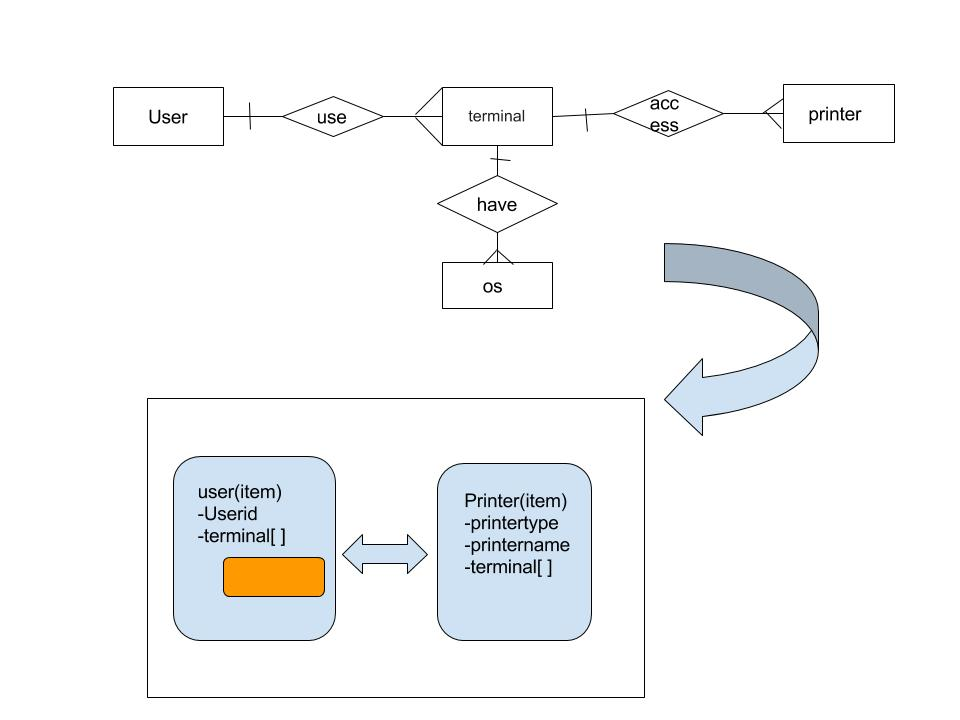
\includegraphics[width=15cm, height=8cm]{2.jpg}
=======
 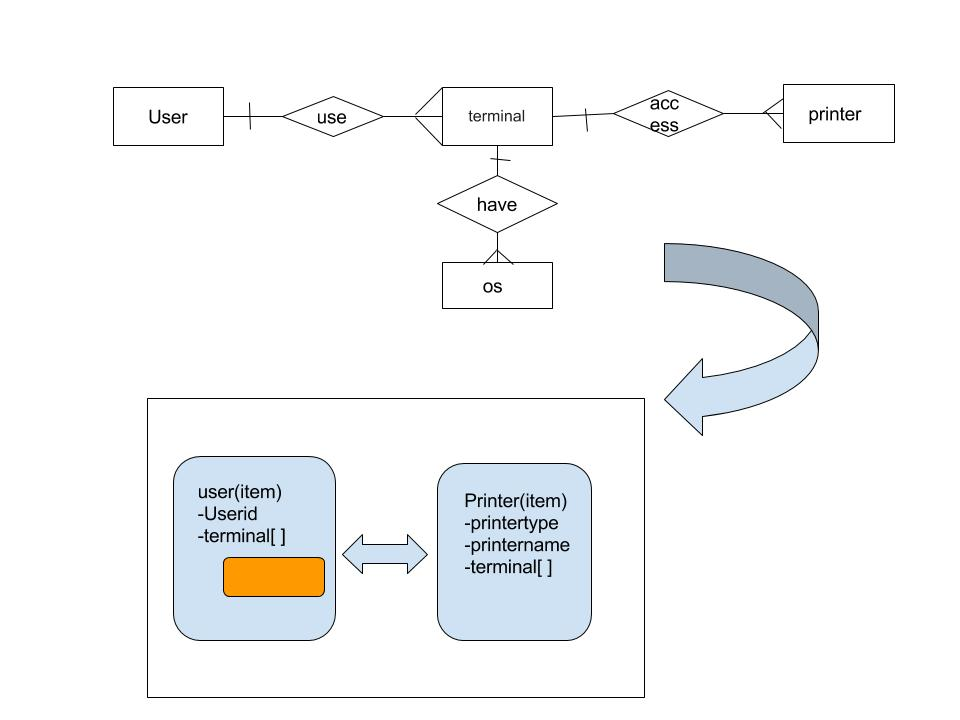
\includegraphics[width=15cm, height=14cm]{2.jpg}
>>>>>>> f404785e3b81514af4d6d2a8723826af43401a12
 \centering
 \caption{\label{fig:1}ER-diagram to NoSQL database table}
 \end{figure}

    \subsection{Algorithm viewpoint}
    Algorithm viewpoint will be use to implement different operation such as create table, upload data, update table, delete table, list table, query table and scan table.\\
\\
    Design concerns\\
    The concern for this part will be how to design the algorithm for operations. Fortunately, the Amazon provides basic APIs for the operations. So we can adapt it from the Amazon document API.\\
\\
    APIS for operation\\
    (1) Create Tables\\
    We will use the AWS SDK for creating tables. The Amazon provides the Java document API for creating tables.These API will help us to create the database schema that we need.The API will first create a dynamoDB class. After that it declares a table request which contains the table name, key of table, the definitions of attributes and capacity.\\
    Here is the API\cite{w1} :\\
<<<<<<< HEAD
    \begin{lstlisting}[caption=API for create tables]
	DynamoDB dynamoDB = new DynamoDB(new Client(new Provider()));
	ArrayList [Attribute] attribute= new ArrayList[Attribute] ();
	attribute.add(new Attribute().withAttributeName("Id").withAttributeType("N"));
  	ArrayList[Element] key = new ArrayList[Element] ();
 	key.add(new  Element().withAttributeName("Id").withKeyType(KeyType.HASH));
	CreateTableRequest request = new CreateTableRequest()
	.withTableName(table)
	......
	.withProvisionedThroughput(new ProvisionedThroughput()
	.withReadCapacityUnits(size)
	.withWriteCapacityUnits(size));
	Table table = dynamoDB.createTable(request);
	table.waitForActive();
  \end{lstlisting}
    (2) Upload Data\\
    We will use the AWS SDK for uploading data into schema. The Amazon provides the Java document API for uploading data.We will use these API to upload the data into the table that we create. The API will first create dynamoDB class.After that it declares a new item which contains the primary key, string set and the numbers for uploading.\\
    Here is the API\cite{w1}:\\
    \begin{lstlisting}[caption=API for Upload data]
    Table table = dynamoDB.getTable(Name);
    try 
    Item item = new Item()
           .withPrimaryKey(Key)
           .withString(string)
           .withNumber(number)
           .withBoolean()
           ....
           .withString();
    table.putItem();
  \end{lstlisting}
    (3) Update Table\\
    We will use the AWS SDK for updating table. The Amazon provides the Java document API for updating table.We will use these API to update the data in the table that we create.The API will first create table class. After that it declares a new class called “provisionedthroughput” which contains the information for updating.\\
    Here is the API\cite{w1}:
      \begin{lstlisting}[caption=API for update table]
    DynamoDB dynamoDB = new DynamoDB(new Client(
    new Provider()));
    Table table = dynamoDB.getTable(table);
    ProvisionedThroughput provisionedThroughput = new ProvisionedThroughput()
    .withReadCapacityUnits(size)
    .withWriteCapacityUnits(size);
    table.updateTable(provisionedThroughput);
    table.waitForActive();
\end{lstlisting}
    (4) Delete Table\\
    We will use the AWS SDK for deleting table. The Amazon provides the Java document API for deleting table. We will use these API to deleting table. The API will create table class. After that, it deletes the table which is the table need to delete.\\
    Here is the API\cite{w1}:
      \begin{lstlisting}[caption=API for delete data]
    DynamoDB dynamoDB = new DynamoDB(new Client(
    new Provider()));
    Table table = dynamoDB.getTable(table);
    table.delete();
    table.waitForDelete();
	\end{lstlisting}
    (5) List table\\
    We will use the AWS SDK for listing table. The Amazon provides the Java document API for listing table.We will use these API to list the data in the table that we create.The API will first create DynamoDB class. After that it will execute the list table method for listing table.\\
    Here is the API\cite{w1}:\\
     \begin{lstlisting}[caption=API for list table]
    DynamoDB dynamoDB = new DynamoDB(new Client(new Provider()));
    TableCollection[Result] tables = dynamoDB.listTables();
    Iterator[Table] iterator = tables.iterator();
    while (iterator.hasNext()) 
    Table table = iteratornext();
    System.out.println(table.getTableName());
    \end{lstlisting}
    (6) Query table \\
    We will use the AWS SDK for query the table. The Amazon provides the Java document API for querying the table.We will use these API to query the table that we create. The API will first create DynamoDB class.Then, it will create a table class which use to represent the table for retrieving. After that, it will use the query to retrieving the data.\\
    Here is the API\cite{w2}:
      \begin{lstlisting}[caption=API for query table]
    DynamoDB dynamoDB = new DynamoDB(
    new Client(new Provider()));
    Table table = dynamoDB.getTable(table);
    QuerySpec spec = new QuerySpec()
    .withValueMap(new ValueMap()
    ItemCollection[Query] items = table.query(spec);
    Iterator[Item] iterator = items.iterator();
    Item item = null;
    while (iterator.hasNext()) {
    item = iterator.next();
    System.out.println(item.toJSONPretty());
	\end{lstlisting}
    (7) Scan Table \\
    We will use the AWS SDK for scan the table.The Amazon provides the Java document API for scan the table.We will use these API to scan the table in order to read the data which store in the table. The API will create a class called “Client”. Then, it create a class which use to provide the information of table for scanning.\\
    Here is the API for Scan Table\cite{w3}:
      \begin{lstlisting}[caption=API for scan table]
    AmazonDynamoDBClient client = new Client(
    new Provider());
    ScanRequest scanRequest = new ScanRequest()
    .withTableName(table);
    ScanResult result = client.scan(Request);
    for (Map[String, Attribute] item : result.getItems()){
    printItem(item);}
    \end{lstlisting}
=======
    DynamoDB dynamoDB = new DynamoDB(new Client(
    new Provider()));\\
    ArrayList [Attribute] attribute= new ArrayList[Attribute] ();\\
    attribute.add(new Attribute().withAttributeName("Id").withAttributeType("N"));\\
    ArrayList[Element] key = new ArrayList[Element] ();\\
 key.add(new  Element().withAttributeName("Id").withKeyType(KeyType.HASH));\\
CreateTableRequest request = new CreateTableRequest()\\
.withTableName(table)\\
......\\
.withProvisionedThroughput(new ProvisionedThroughput()\\
            .withReadCapacityUnits(size)\\
            .withWriteCapacityUnits(size));\\
    Table table = dynamoDB.createTable(request);\\
    table.waitForActive();\\
\\
    (2) Upload Data\\
    We will use the AWS SDK for uploading data into schema. The Amazon provides the Java document API for uploading data.We will use these API to upload the data into the table that we create. The API will first create dynamoDB class.After that it declares a new item which contains the primary key, string set and the numbers for uploading.\\
    Here is the API\cite{w1}:\\
    Table table = dynamoDB.getTable(Name);\\
    try \\
    Item item = new Item()\\
                 .withPrimaryKey(Key)\\
                 .withString(string)\\
                 .withNumber(number)\\
                 .withBoolean()\\
                 ....\\
                 .withString();\\
    table.putItem();\\
\\
    (3) Update Table\\
    We will use the AWS SDK for updating table. The Amazon provides the Java document API for updating table.We will use these API to update the data in the table that we create.The API will first create table class. After that it declares a new class called “provisionedthroughput” which contains the information for updating.\\
    Here is the API\cite{w1}:\\
    DynamoDB dynamoDB = new DynamoDB(new Client(
    new Provider()));\\
    Table table = dynamoDB.getTable(table);\\
    ProvisionedThroughput provisionedThroughput = new ProvisionedThroughput()
    .withReadCapacityUnits(size)\\
    .withWriteCapacityUnits(size);\\
    table.updateTable(provisionedThroughput);\\
    table.waitForActive();\\
\\
    (4) Delete Table\\
    We will use the AWS SDK for deleting table. The Amazon provides the Java document API for deleting table. We will use these API to deleting table. The API will create table class. After that, it deletes the table which is the table need to delete.\\
    Here is the API\cite{w1}:\\
    DynamoDB dynamoDB = new DynamoDB(new Client(
    new Provider()));\\
    Table table = dynamoDB.getTable(table);\\
    table.delete();\\
    table.waitForDelete();\\
\\
    (5) List table\\
    We will use the AWS SDK for listing table. The Amazon provides the Java document API for listing table.We will use these API to list the data in the table that we create.The API will first create DynamoDB class. After that it will execute the list table method for listing table.\\
    Here is the API\cite{w1}:\\
    DynamoDB dynamoDB = new DynamoDB(new Client(
       new Provider()));\\
    TableCollection[Result] tables = dynamoDB.listTables();\\
    Iterator[Table] iterator = tables.iterator();\\
    while (iterator.hasNext()) \\
    Table table = iteratornext();\\
    System.out.println(table.getTableName());\\
\\
    (6) Query table \\
    We will use the AWS SDK for query the table. The Amazon provides the Java document API for querying the table.We will use these API to query the table that we create. The API will first create DynamoDB class.Then, it will create a table class which use to represent the table for retrieving. After that, it will use the query to retrieving the data.\\
    Here is the API\cite{w2}:\\
    DynamoDB dynamoDB = new DynamoDB(
    new Client(new Provider()));\\
    Table table = dynamoDB.getTable(table);\\
    QuerySpec spec = new QuerySpec()\\
    .withValueMap(new ValueMap()\\
    ItemCollection[Query] items = table.query(spec);\\
    Iterator[Item] iterator = items.iterator();\\
    Item item = null;\\
    while (iterator.hasNext()) {\\
    item = iterator.next();\\
    System.out.println(item.toJSONPretty());\\
\\
    (7) Scan Table \\
    We will use the AWS SDK for scan the table.The Amazon provides the Java document API for scan the table.We will use these API to scan the table in order to read the data which store in the table. The API will create a class called “Client”. Then, it create a class which use to provide the information of table for scanning.\\
    Here is the API for Scan Table\cite{w3}:\\
    AmazonDynamoDBClient client = new Client(
    new Provider());\\
    ScanRequest scanRequest = new ScanRequest()\\
    .withTableName(table);\\
    ScanResult result = client.scan(Request);\\
    for (Map[String, Attribute] item : result.getItems()){\\
    printItem(item);}\\
>>>>>>> f404785e3b81514af4d6d2a8723826af43401a12
\section{Quicksight}
    \subsection{Overview}
    The data store in the DynamoDB will be used to create an analyze and a visual on Amazon visualization tool called Quicksight. In this part, Information viewpoint will be used.
    \subsection{Information viewpoint}
    The information viewpoint can be used to achieve visualization part. Basically, we will use the Quicksight as the visualization tool to represent the analyzing result.\\
\\
    Design concern \\
    The major concern for this part will be how to generate a visual on the Quicksight. Fortunately, the Amazon provides tutorial on the Quicksight document. Therefore, we can a follow the instruction step by step from the document.\\
\\    
    Step for creating a visual\\
    Base on the Quicksight document, there will be several general step for creating a visual. The first step is to create a data source in your database. These data source are very important for Quicksight because it will require these data source for creating data set and do the analyzing. After that, the Quicksight needs to connect with the data source. In this step, if the database is on the Amazon web services the data source will be easily to connect. However, if the data source is not on the Amazon web services it requires port, database access information to connect the data source in database. The detail information is on the Amazon Quicksight document. The next step is to create the data set according to data source and do an analyzing. The last step is to create a visual according to the data set. There are different types of visual on the Quicksight and we can choose one to generate the suitable graph for the analyzing result.\cite{w4}\\
The figure \ref{fig:2} is the general process:
    \begin{figure}[h]
<<<<<<< HEAD
    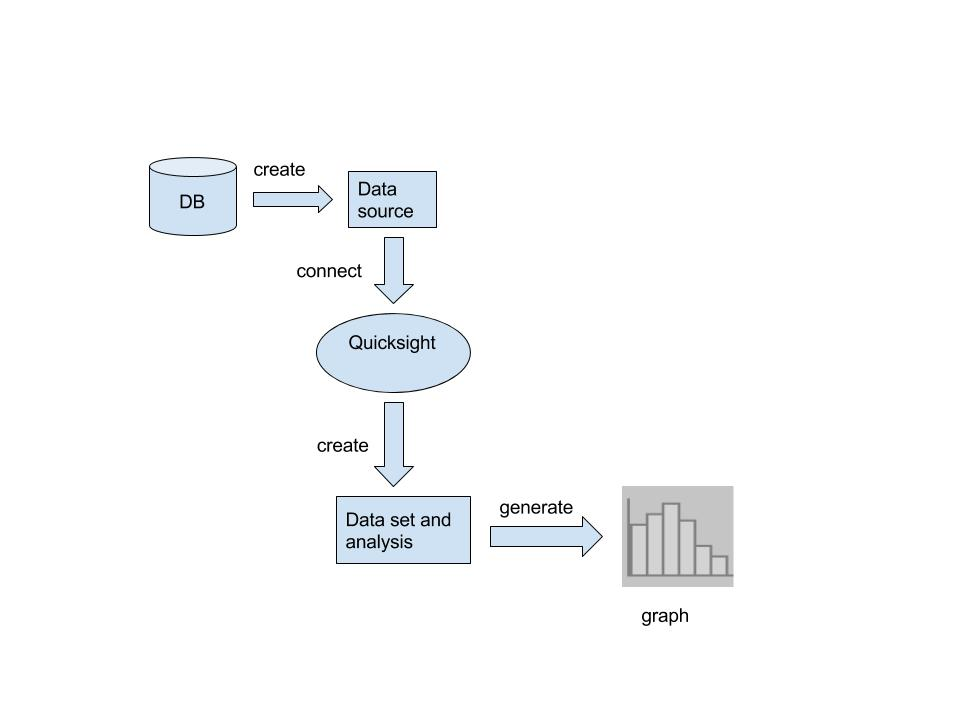
\includegraphics[width=16cm, height=8cm]{4.jpg}
    \centering
    \caption{\label{fig:2}General process}
    \end{figure}
=======
    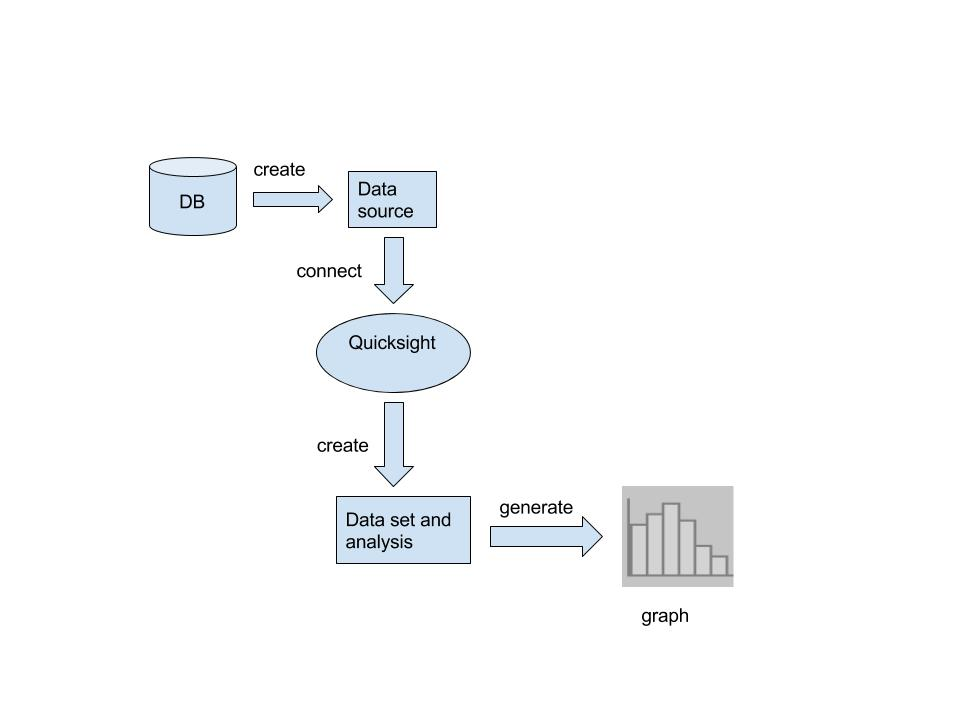
\includegraphics[width=18cm, height=8cm]{4.jpg}
    \centering
    \caption{\label{fig:2}General process}
    \end{figure}
>>>>>>> f404785e3b81514af4d6d2a8723826af43401a12
